\chapter{Background}
\label{chap:backgroud}

In this chapter, we will introduce some basic terminology as well as provide further information surrounding carbon scheduling.

\paragraph{The Composition of the Public Grid}

As outlined in the previous chapter, there is a diurnal rhythm to the renewable energy production.
In addition to that, there is also a seasonal effect on the energy grid composition:
As shown in Figure \ref{fig:energy_mix_year}, during warm seasons (e.g. July), more solar is produced than in colder seasons, and the share in renewables rises accordingly.

\begin{figure}
    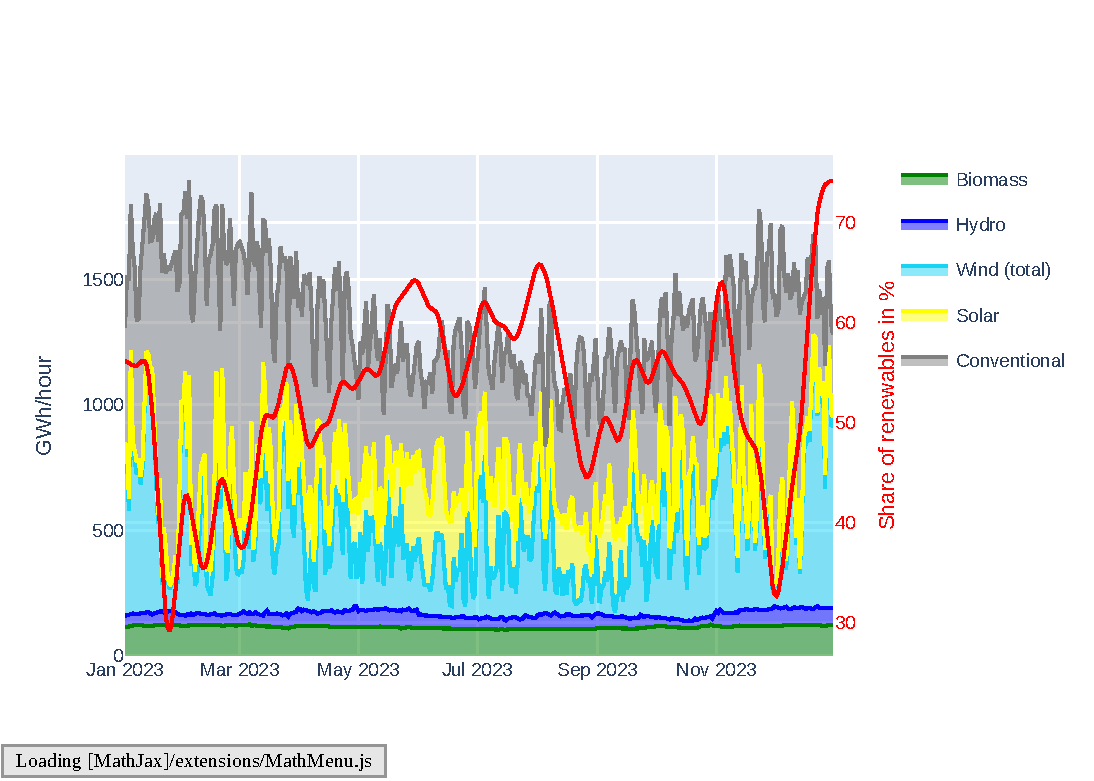
\includegraphics[width=\linewidth]{agorameter/energy_production_year.pdf}
    \caption[short]{Mix of energy production in Germany in 2023. Data provided by \url{agora-energiewende.org}}
    \label{fig:energy_mix_year}
\end{figure}

The demand for power also has an effect on the overall composition. 
During times of low demand, less conventional power needs to be produced and renewables have a higher share as well.
This can be seen in the seasonal Figure: during Christmas holidays in December, people spend more time at home, requiring less additional conventional energy (e.g. for industrial consumers, as people also work less).

All the above is a local or national view on the public grid. 
When looking at energy production globally, a spatial dimension is added. 
This takes effect in the form of different countries having peak solar production at different times (following the earth's rotation), but also takes effect in the composition of production capabilities.
Some countries may have less investment in renewables or may use nuclear power plants, which are also deemed low-carbon\todo{Needs citation} but have less of a seasonal or diurnal rhythm (if they are not limited by lack of cooling water\footnote{\url{https://www.euronews.com/green/2023/07/13/frances-nuclear-power-stations-to-limit \allowbreak -energy-output-due-to-high-river-temperatures}}).\todo{Needs to be integrated better xd}

Thus, as outlined by \cite{wiesner_lets_2021}, national public grids have a certain affinity for carbon aware scheduling. Generally, the higher the solar capacities, the higher the potential carbon saving from such an approach. 

\paragraph{Power Grid Signals}
Carbon-aware scheduling commonly works on two possible metrics or signals: the \emph{average emissions} are the metric describing the amount of carbon per unit of energy, basically what has been used in the text so far. Another metric is the \emph{marginal emissions}, answering the question of "if more energy is used at this point in time, how much carbon would that cost?". 
The answer to that question is usually that non-renewable power plants have to increase production as renewable sources cannot increase production to meet demand (as the sun and wind intensity are set by the weather). 
Going by the marginal metric, any kind of carbon aware scheduling is pointless, as any work at any point in time results in the same increase of carbon. 
There are, however, secondary reasons that render carbon-aware scheduling useful still. 
One of them are is \emph{curtailment}. 
Curtailment encompasses any methods that reduce the amount of produced renewable energy. As the power grid always needs to have a balance between demand and production, curtailment methods such as turning of wind turbines, selling power at a loss, or charging batteries may be used. 
Carbon aware scheduling via the average emissions signal lowers the amount of curtailment needed, as demand for energy would increase at those times.
Another argument made, for example by Fridgen et al. \cite{fridgen_not_2021}, is that by increasing power demand during times when renewable production is high, investments in renewables would be promoted. 
Lastly, as renewable energy is generally cheaper in production than non-renewable energy\todo{Need a citation here!}, scheduling work on low carbon-periods coincides with cheaper energy prices as well. While this would not reduce costs on most energy contracts, there are also some contracts that use dynamic pricing \footnote{One example for dynamic pricing is \emph{Tibber}: \url{tibber.com}}

\paragraph{Workloads in a Datacenter} According to Tanenbaum and Woodhull \cite{tanenbaum_operating_2006}, there are three environments in which scheduling may take place. \emph{Batch systems} describe environments in which there is no user interaction.
A user may submit their job, and it would be executed according to the scheduler at some point in time. \todo{Does this need more examples?}
On the contrary, in \emph{interactive} settings, a user interacts with the system, and thus expects quick responses to their inputs. 
The last environment are \emph{real time} systems. There, deadlines and predictability dictate how a scheduler operate.

For this work's topic, carbon-aware scheduling, only batch systems will be looked at as they allow more freedom to the times of scheduled jobs. 

\todo{I could also add more stuff about metrics and so on, but I am not using them yet in my implementation}

Which metrics are there POI-A, etc.

\paragraph{Power Intake of a Computer}
As there will be power measurements in \ref{sec:power_measurements}, some basic understanding of energy and power used for computation will be provided:
\begin{itemize}
    \item I could mostly borrow from the EBRH slides; there is some base power needed that is correlated to the hardware (dynamic and static energy)
    \item this also depends on frequency (which is why later we set our CPU frequency to some hard coded value [or do not do that in the case of my GPU lol])
    \item basically, use this paragraph to outline all things we take care of in my power measurements
\end{itemize}

\paragraph{Measuring Power}

There are multiple options for measuring the power of a given computer. One way of classifying these options would be under them being either \emph{logical measurements} or \emph{physical measurements}.

Logical ones would create a model on some metrics and derive the used power. One example would be using Linux' \emph{perf} tool to read hardware performance counters. \todo{This needs some more here}

Advantages of choosing a logical approach would be that no external hardware is needed and that the overhead of the measurement would be low, as the hardware counters are being kept track of anyway. 
Disadvantages on the other hand would be that such a model would have to be created or chosen and would include some form of error as all models do.

Physical measurements follow another route; measurement devices would be put between the operating hardware and the power supply. 
The point where a power measuring device is inserted would dictate what could and could not be measured, a wall mounted measurement device could only measure all power going into a computer and not differentiate between individual programs.

Advantages of physical measurements are that they can give a more holistic measurement of a system as would be the case for a wall mounted measurement device. 
Portability is an issue however, unlike operating-system supported tools such as perf, a measurement device would need more effort to be used on another system (or be entirely not useable, for example when such devices are only rated for a certain power level).